\documentclass{beamer}

\usepackage{color}
\usepackage{graphicx}
\usepackage{amsmath}

\newcommand{\blue}[1]{\textcolor{blue}{#1}}
\newcommand{\red}[1]{\textcolor{red}{#1}}
\newcommand {\bmu} {\mbox{\boldmath$\mu$}}

\setbeamertemplate{frametitle}[default][center]

\begin{document}

\begin{frame}
\begin{center}
\blue{\Large\bf Triggering Neoclassical Tearing Modes in}\\[0.5ex]
 \blue{\Large\bf NSTX}\\[2ex]
Richard Fitzpatrick\\[0.5ex]
Institute of Fusion Studies, University of Texas at Austin
\end{center}


\end{frame}

\begin{frame}
\frametitle{Motivation}
 
\begin{itemize}
\item Well-known that potentially unstable neoclassical tearing modes (NTMs) in tokamak plasmas are \red{meta-stable}.\footnote{R. Fitzpatrick, 
Phys.\ Plasmas {\bf 2}, 825 (1995).}
\item In other words, such NTMs require some sort of externally applied ``kick'' before they can grow and saturate at large amplitudes.
\item What can provide this kick? 
\item Generally assumed that kick is \red{transient magnetic perturbation} due to other modes that occur in plasma: e.g., sawtooth crashes, edge localized modes, other NTMs, etc.
\item However, there has been very little systematic investigation into what properties a transient magnetic
perturbation needs to possess in order to successfully trigger an NTM. 
\item Present talk reports on first step in such an investigation. 
\end{itemize}
\end{frame}

\begin{frame}
\frametitle{NSTX Shot 127317}
\frametitle{EPEC Code}
 
\begin{itemize}
\item \red{EPEC code} simulates tearing mode dynamics in tokamak plasma using an \red{asymptotic matching} approach.\footnote{R. Fitzpatrick, S.K.~Kim, and J.~Lee, Phys.\ Plasmas {\bf 28}, 082511 (2021).}  
\item Code incorporates magnetic equilibrium data (g-file) and profile data (p-file). 
\item Code includes toroidal coupling between different tearing modes. 
\item Code incorporates accurate neoclassical model that includes impurities and neutrals, and allows calculation of bootstrap
drive to tearing modes.\footnote{S.P.~Hirshman and D.J.~Sigmar, Nucl.\ Fusion {\bf 21}, 1079 (1981).} 
\item For case of NSTX, external perturbation is provided by pulsing RMP coils. However, perturbation is allowed to rotate.
This mimics multi-harmonic rotating magnetic perturbation generated by sawtooth crash, etc.
\end{itemize}
\end{frame}

\begin{frame}
\frametitle{NSTX Shot 127317}
 
\begin{itemize}
\item NSTX shot 127317 was one of the shots used in the experimental campaign  that demonstrated  ELM destabilization via an externally applied non-axisymmetric
resonant magnetic perturbation (RMP).\footnote{J.M.~Canik, et al.\ Nucl.\ Fusion {\bf 50}, 034012 (2010).}
\end{itemize}
\end{frame}

\begin{frame}
\frametitle{NSTX Shot 127317: Magnetic Flux-Surfaces}

\begin{center}
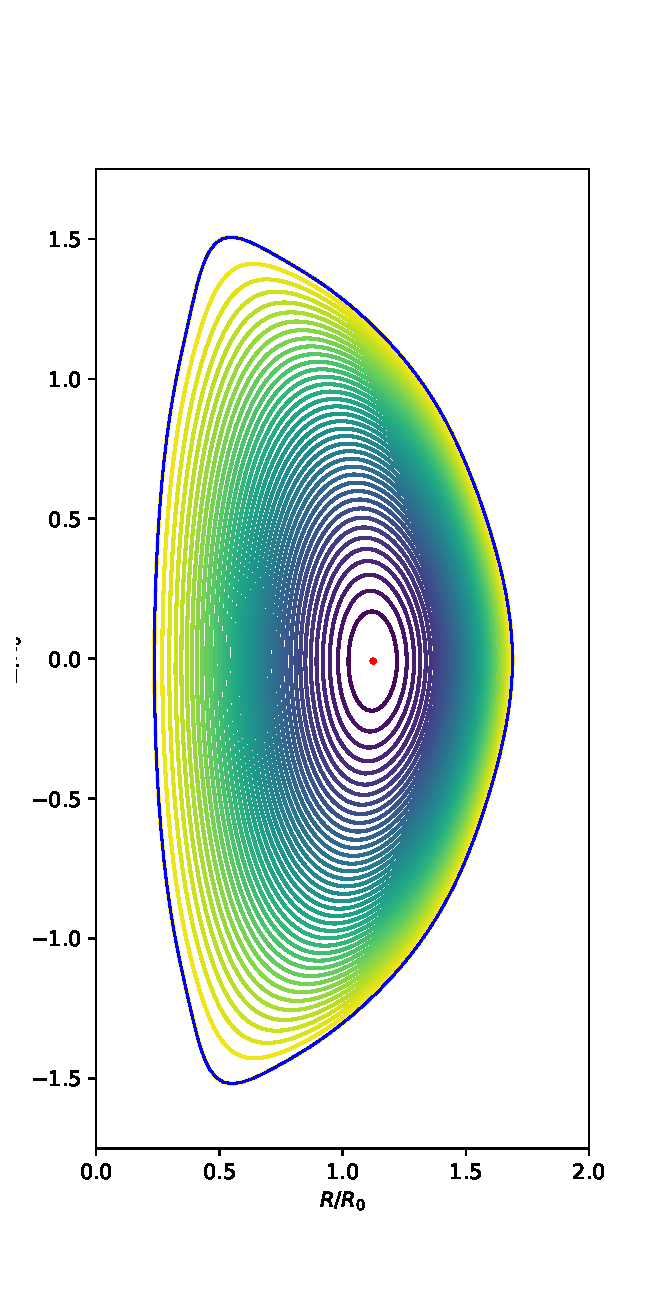
\includegraphics[height=3.5in]{Equilibrium.eps}
\end{center}

\end{frame}

\begin{frame}
\frametitle{NSTX Shot 127317: Profiles}

\begin{center}
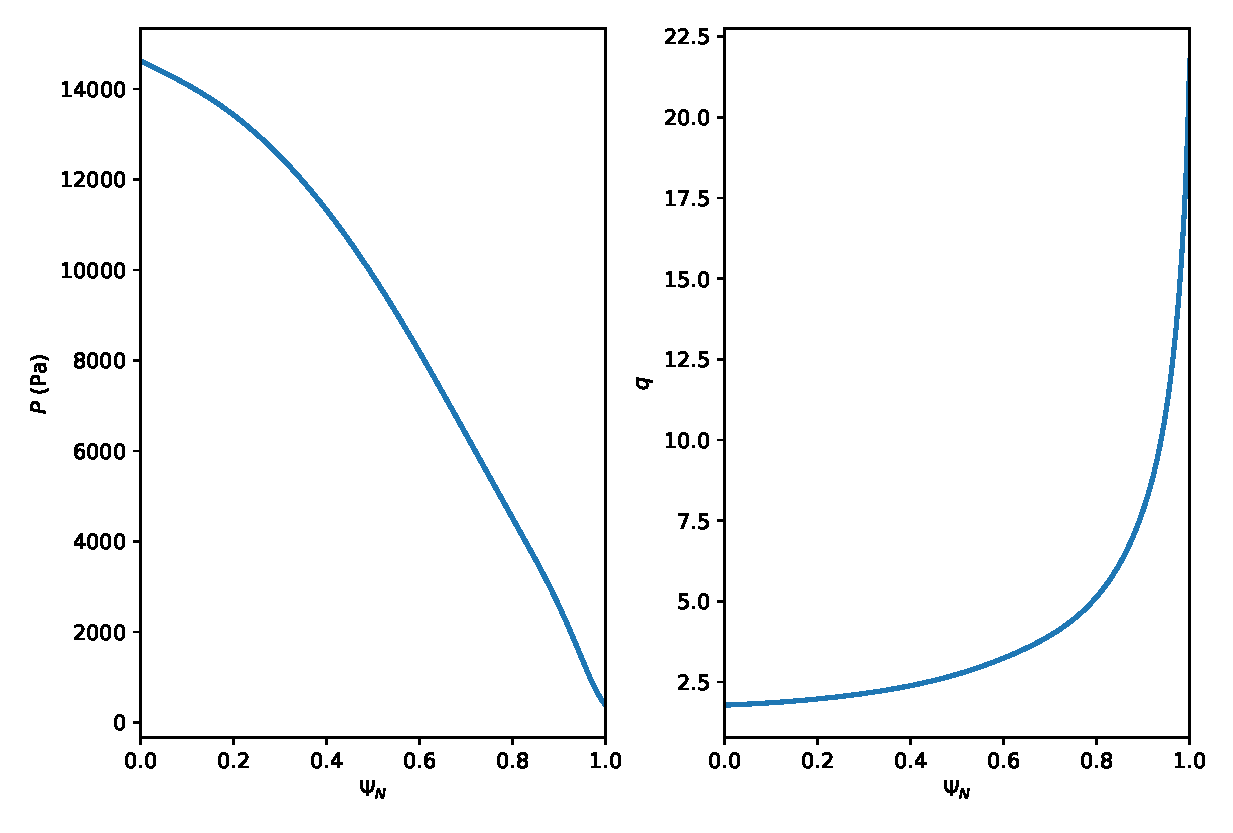
\includegraphics[width=\textwidth]{Profiles.eps}
\end{center}

\end{frame}

\begin{frame}
\frametitle{NSTX Shot 127317: $n=1$ Natural Frequencies}

\begin{center}
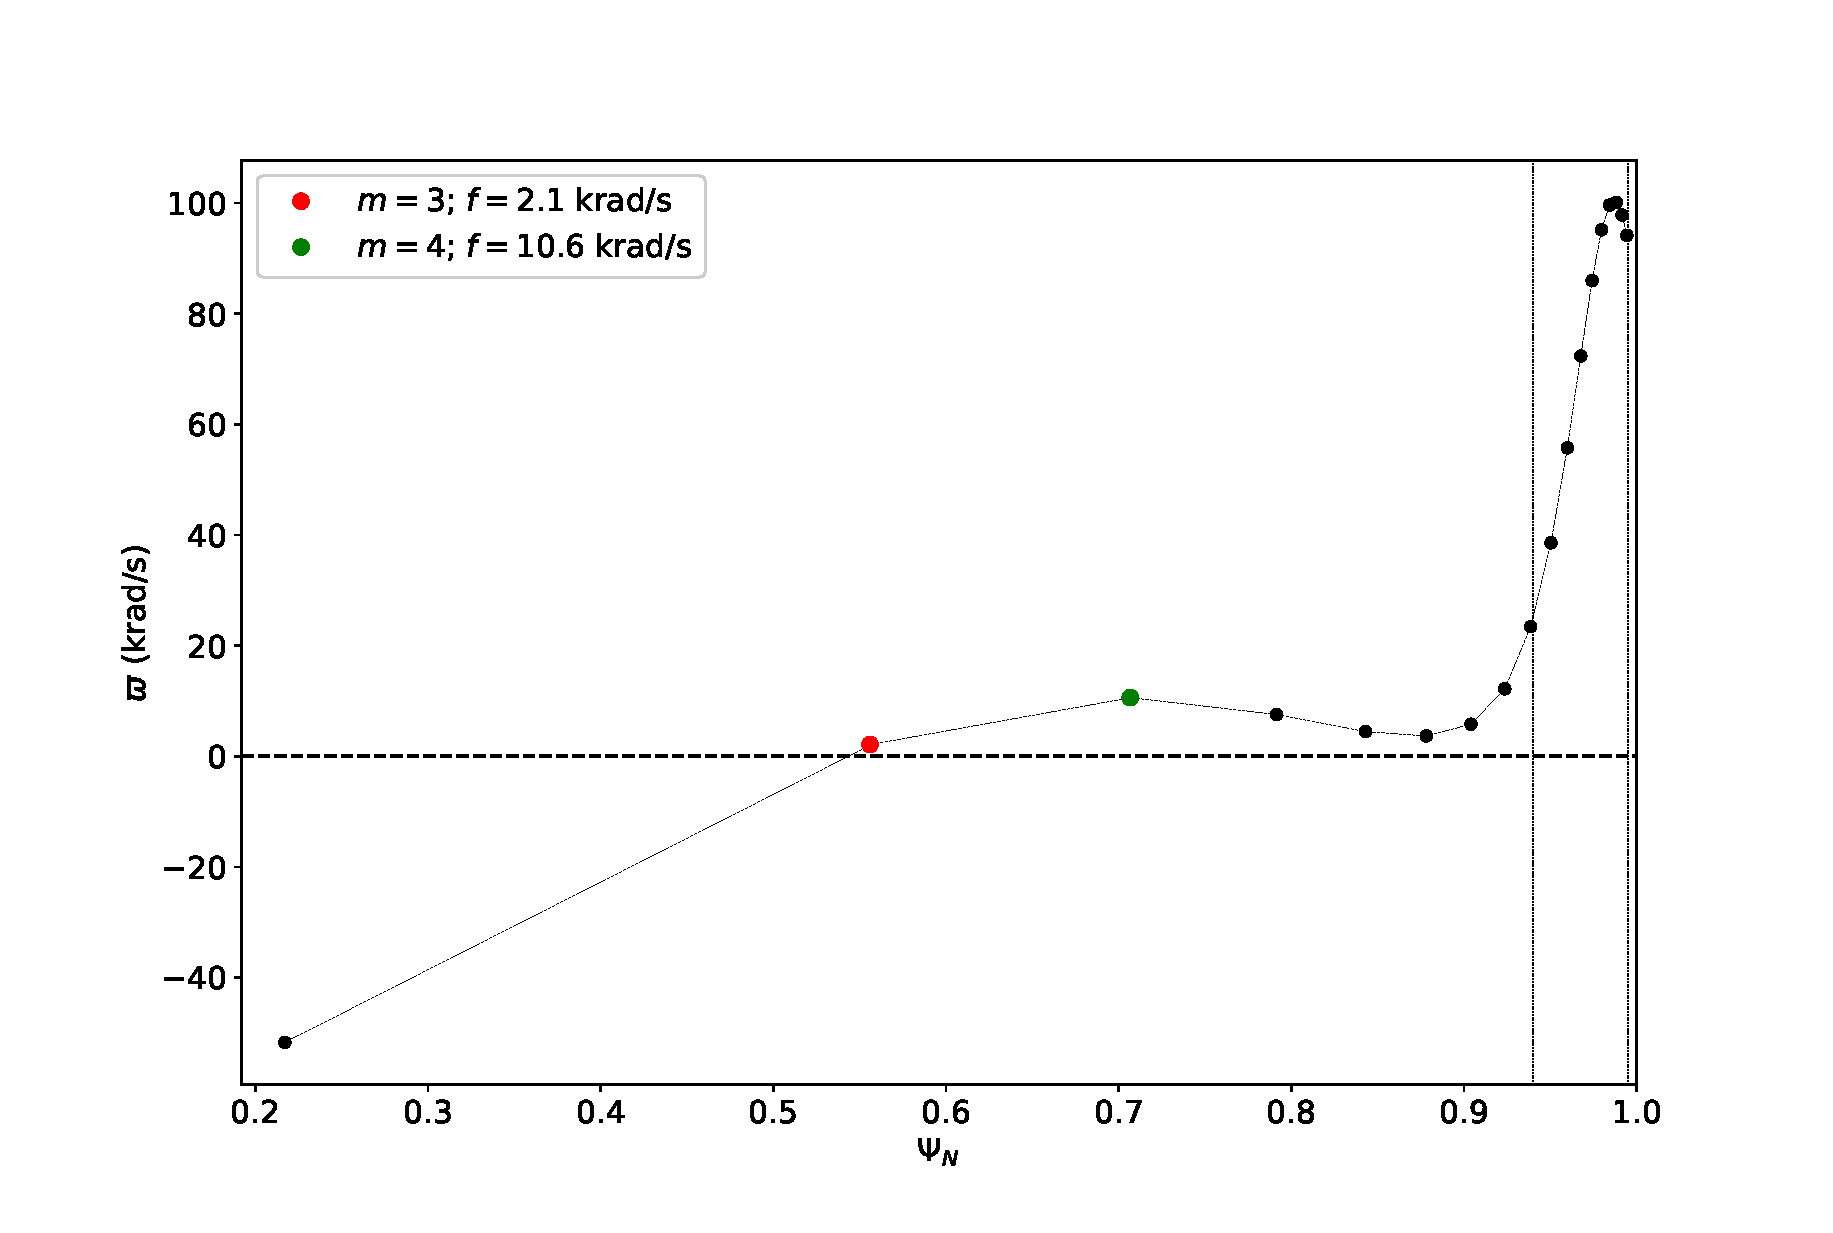
\includegraphics[width=\textwidth]{Frequency.eps}
\end{center}
\end{frame}

\begin{frame}
\frametitle{NSTX Shot 127317: $n=1$ Modes}
\begin{itemize}
\item NSTX shot 127137 (400 ms) contains \blue{18 $n=1$} rational surfaces, corresponding to \blue{$m=2$} through
\blue{$m=19$}. 
\item Only two of these surfaces, \blue{$m=3$} and \blue{$m=4$}, are potentially unstable to NTMs.  
\item The \red{natural frequencies} (i.e., frequencies that modes would rotate at if they were naturally unstable) of
these modes are \blue{2.1 krad/s} and \blue{10.6 krad/s}, respectively. 
\item Natural frequencies determined by \blue{${\bf E}\times {\bf B}$} flows, diamagnetic effects, and neoclassical
effects. 
\item EPEC determines natural frequencies from experimental profile data (p-file). However, since there is no
poloidal rotation data in NSTX, poloidal rotation is given its neoclassical value (including impurities and neutrals). 
\end{itemize}
\end{frame}

\begin{frame}
\frametitle{NSTX Shot 127317: Rutherford Island Equation Rhs}

\begin{center}
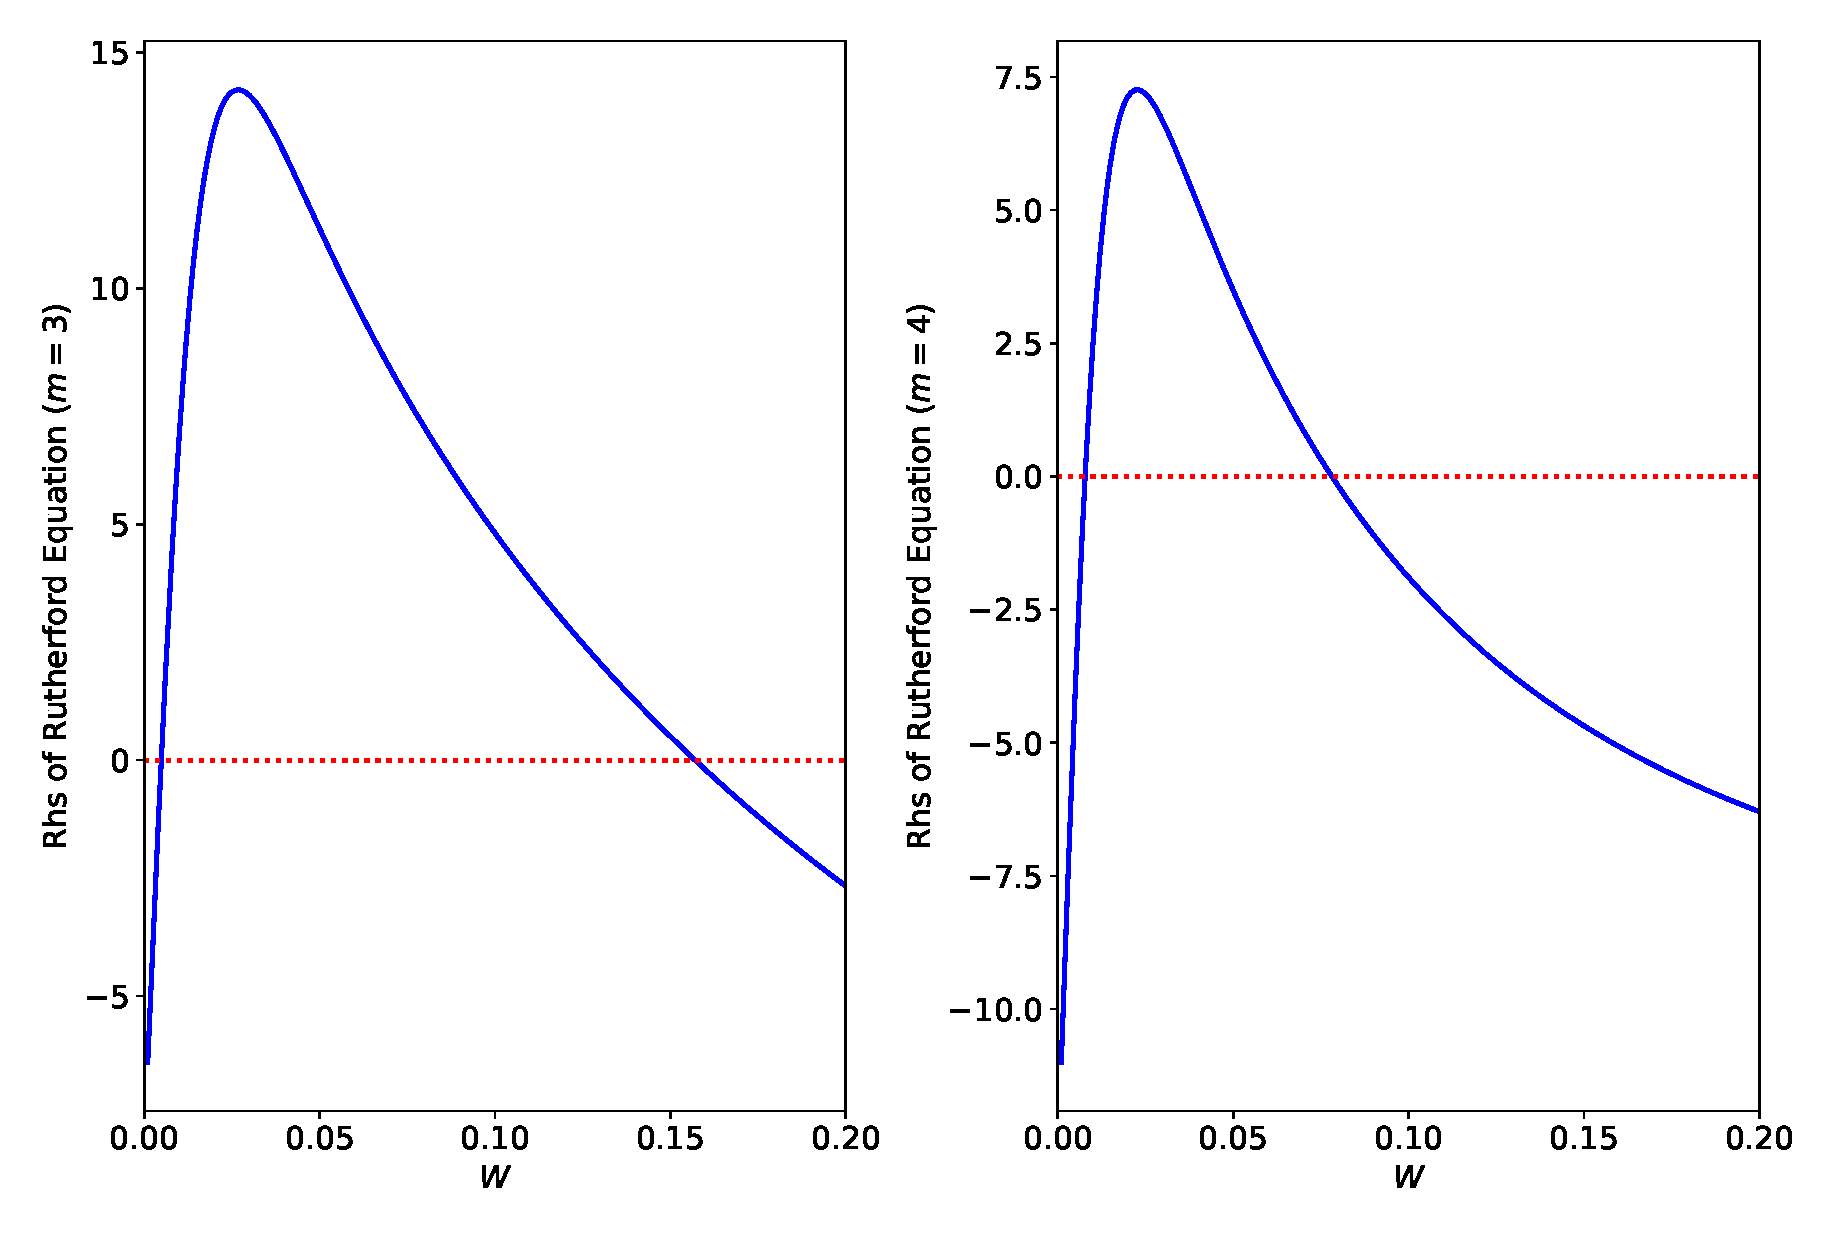
\includegraphics[width=\textwidth]{Rhs.eps}
\end{center}
\end{frame}

\begin{frame}
\frametitle{NSTX Shot 127317: Neoclassical Tearing Modes}

\begin{itemize}
\item Previous figure shows that \blue{$m=3$} and \blue{$m=4$} modes are meta-stable NTMs.
\item Both modes have potential to grow to large amplitudes (\blue{$W\sim 0.16$} and \blue{$W\sim 0.08$}, respectively,  in units
of \blue{${\mit\Psi}_N$}). 
\item No other \blue{$n=1$} modes in plasma have Rutherford equation right-hand sides that rise above zero (i.e.,
they are all intrinsically stable).
\end{itemize}
\end{frame}

\begin{frame}
\frametitle{NSTX Shot 127317: External Perturbation}
\begin{itemize}
\item According to EPEC, if \blue{$n=1$} simulation started in initial state in which all modes have very small
amplitudes then mode amplitudes remain very small indefinitely. In other words, unperturbed plasma is
stable.
\item Apply external magnetic perturbation to system by applying square-wave \blue{$n=1$} current pulse to RMP coils. 
\item Pulse has three properties:
\begin{itemize}
\item Amplitude - \blue{$I_{rmp}(kA)$}.
\item Temporal extent (period)  - \blue{$\tau$(ms)}.
\item Phase velocity - \blue{$f$(krad/s)}.
\end{itemize}
\item How do these properties affect ability of pulse to trigger NTMs?
\end{itemize}

\end{frame}

\begin{frame}
\frametitle{NSTX Shot 127317: Failed NTM Excitation}
\begin{center}
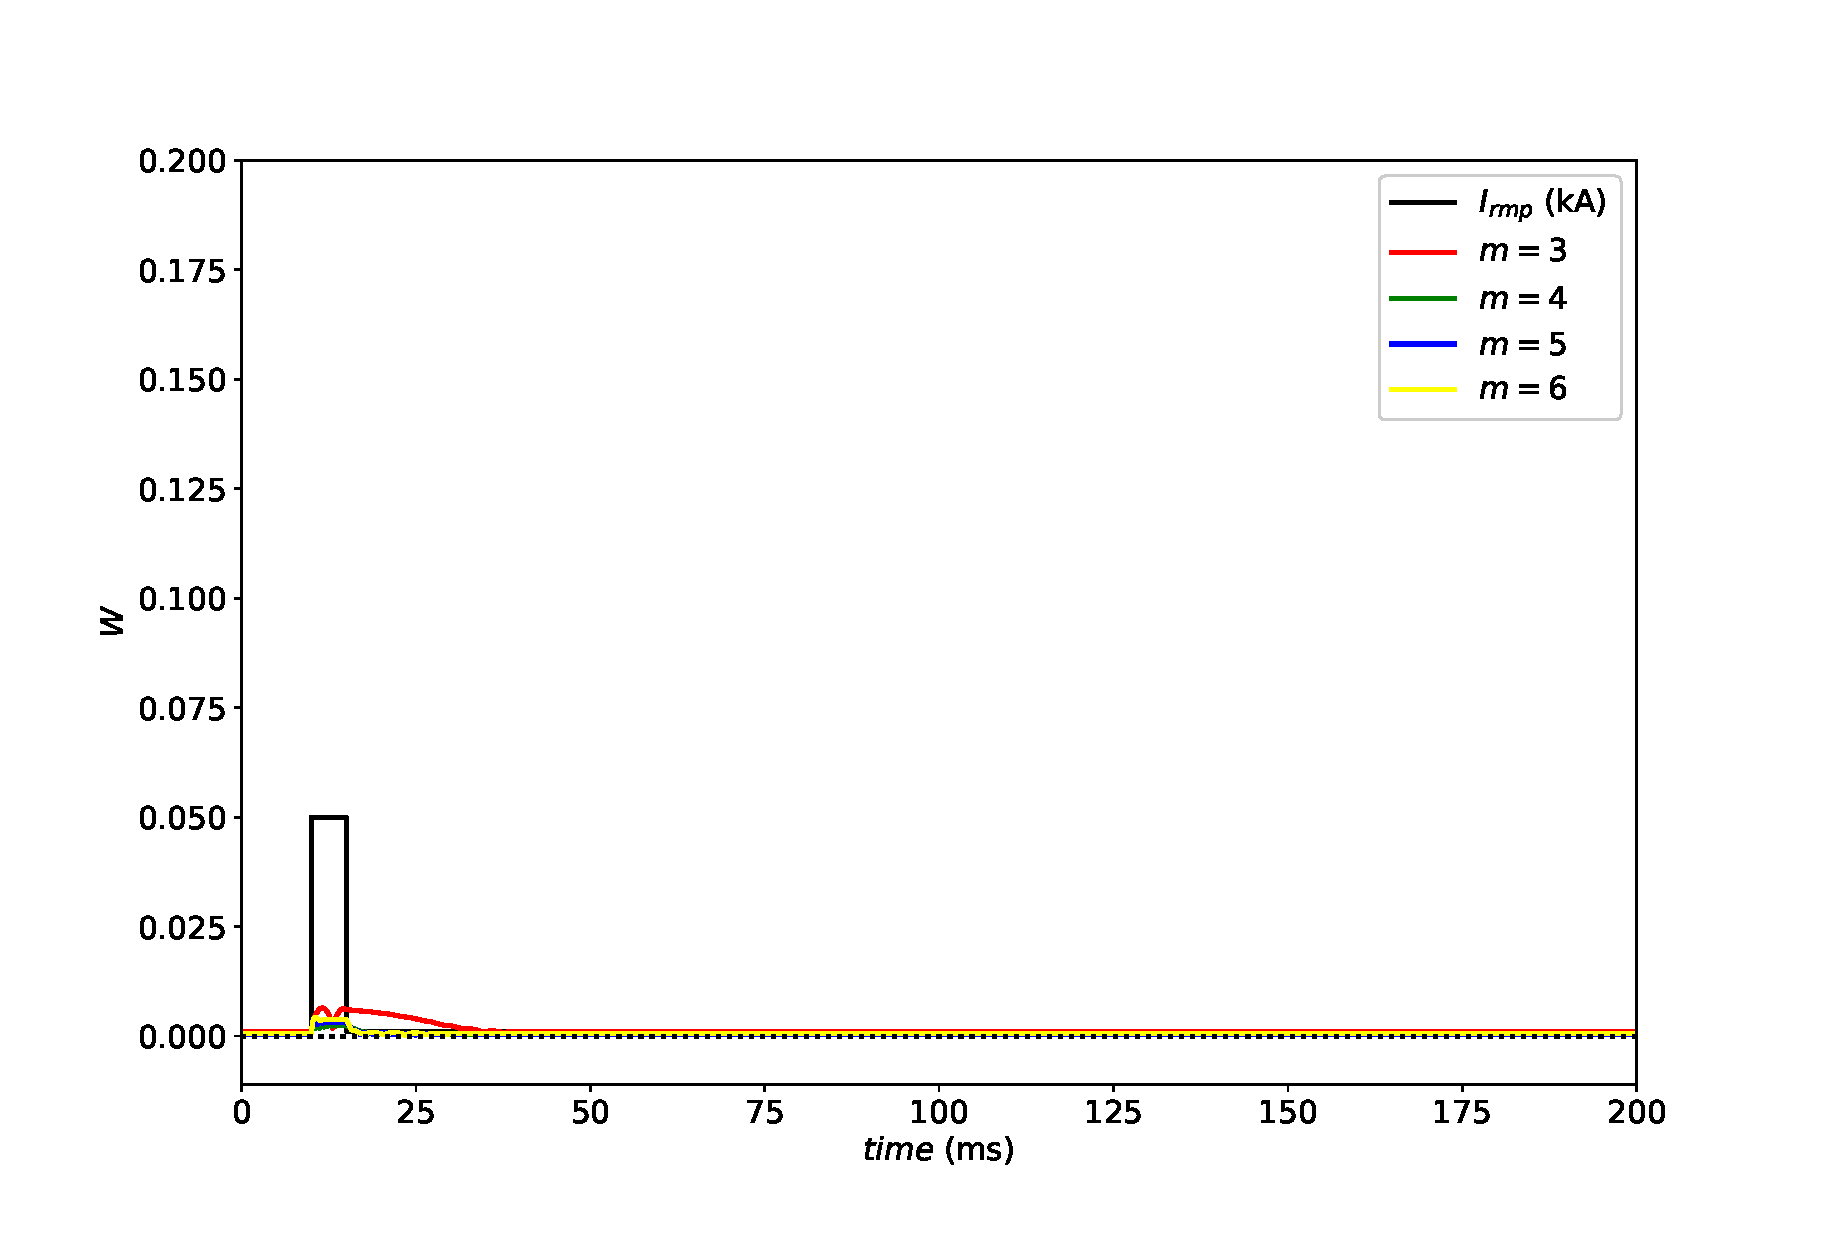
\includegraphics[width=\textwidth]{Waveform0.eps}
\end{center}

\end{frame}

\begin{frame}
\frametitle{NSTX Shot 127317: Failed NTM Excitation}
\begin{itemize}
\item Figure shows a 5 ms period, zero frequency [i.e., \blue{$\tau=5$ (ms)}, \blue{$f= 0$ (krad/s)}] RMP
pulse that  fails to excite an NTM. 
\end{itemize}
\end{frame}

\begin{frame}
\frametitle{NSTX Shot 127317: Successful  NTM Excitation}
\begin{center}
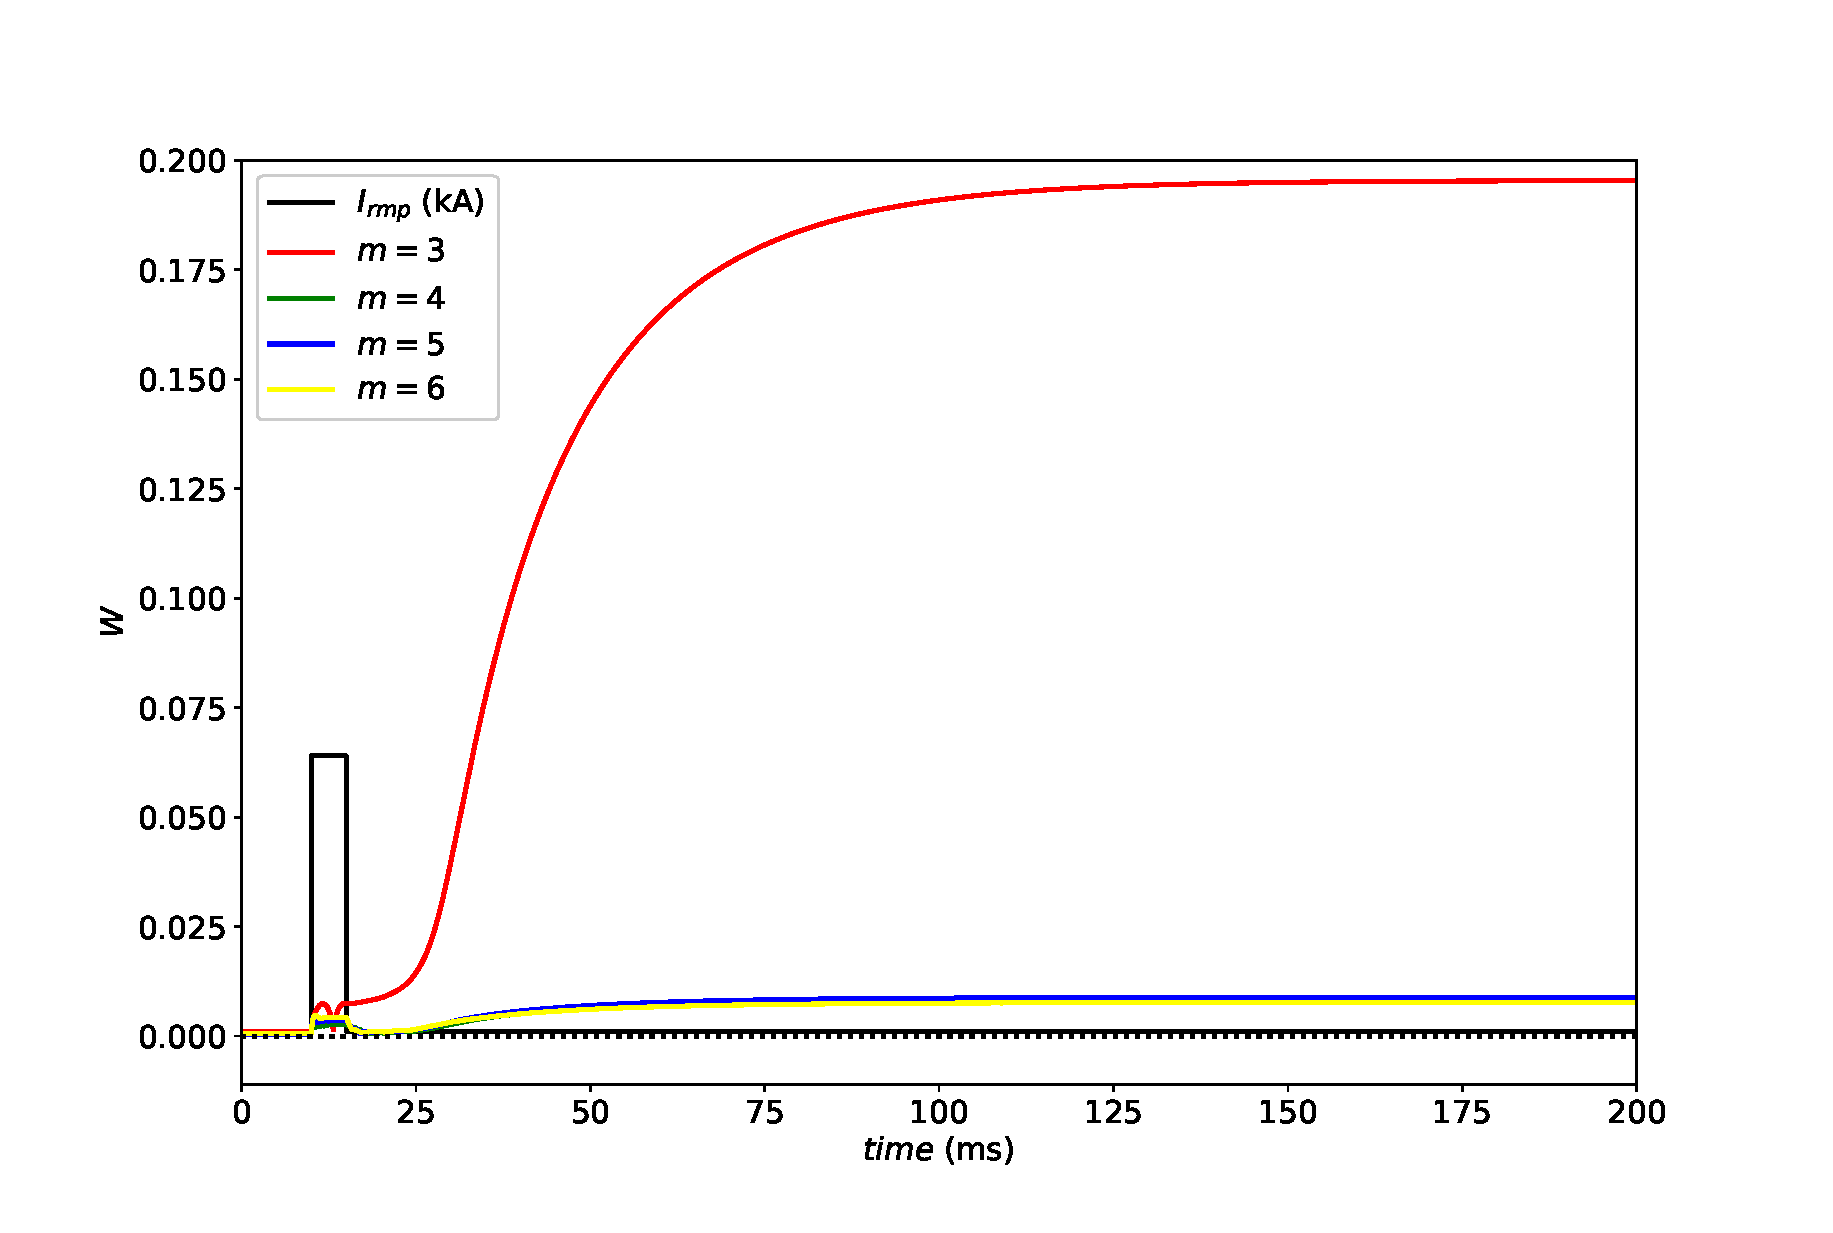
\includegraphics[width=\textwidth]{Waveform1.eps}
\end{center}

\end{frame}

\begin{frame}
\frametitle{NSTX Shot 127317: Successful NTM Excitation}
\begin{itemize}
\item Figure shows a slightly higher amplitude 5 ms period, zero frequency [i.e., \blue{$\tau=5$ (ms)}, \blue{$f= 0$ (krad/s)}] RMP
pulse that  excites an \blue{$m=3$} NTM. 
\item Note that once the \blue{$m=3$} mode grows to high amplitude it acts like an RMP that drives small-amplitude
islands at the \blue{$m=4$, 5, 6} rational surfaces.
\item However, \blue{$m=4$} NTM is not triggered, even after \blue{$m=3$} mode grows to large amplitude. 
\end{itemize}
\end{frame}

\begin{frame}
\frametitle{Period Scan}
\begin{itemize}
\item How does critical RMP current needed to trigger \blue{$m=3$} NTM depend on temporal extent of
RMP pulse? 
\item Would generally expect long pulses to be more effective at driving RMPs than short pulses.
\item So is the dependence just a monotonic decrease with increasing period?
\end{itemize}
\end{frame}

\begin{frame}
\frametitle{EPEC Period Scan}
\begin{itemize}
\item Period scan performed as follows. 
\item Each EPEC run simulates \blue{200 ms}. 
\item At end of run, EPEC determines whether NTM
has been excited or not. 
\item Generally takes \blue{10} to \blue{20} runs to accurately determine critical RPM current (EPEC uses
bisection method). 
\item There are \blue{2000} points in each period-scan curve. 
\item So period-scan curve corresponds to \blue{8000} seconds of simulation.  This would be impossible with
conventional MHD code. However, calculation can be done on ordinary desktop with asymptotic matching approach.
\end{itemize}
\end{frame}


\begin{frame}
\frametitle{NSTX Shot 127317: Period Scan}
\begin{center}
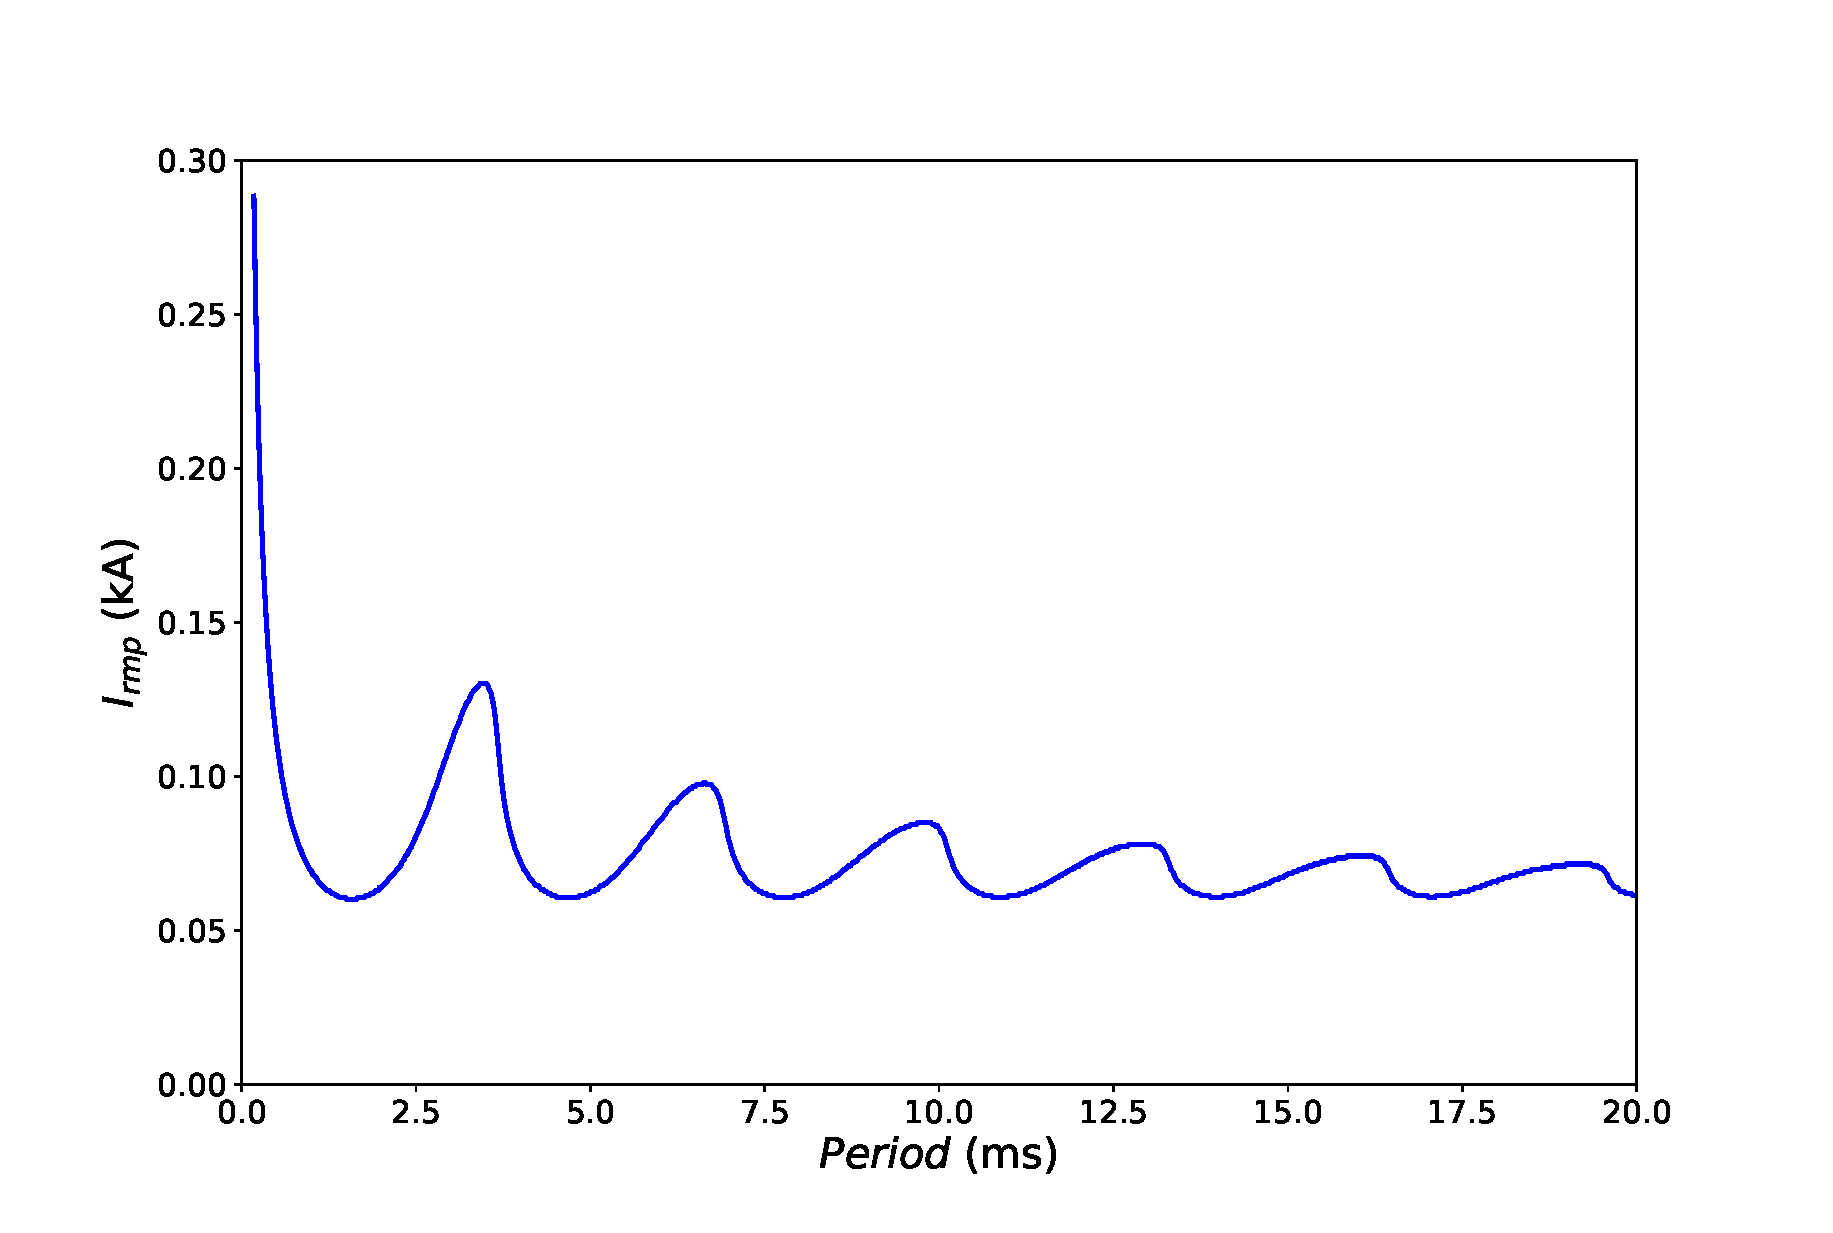
\includegraphics[width=\textwidth]{PeriodScan0.eps}
\end{center}

\end{frame}

\begin{frame}
\frametitle{NSTX Shot 127317: Period Scan}
\begin{itemize}
\item Figure shows critical RMP current required to trigger \blue{$m=3$} NTM as function of pulse temporal extent (period).
Pulse is non-rotating. 

\item On average, critical RMP current does indeed go down with increasing pulse period.
\item However, critical RMP current has unexpected oscillations. 
\item Note that all minima are same. Implies that \blue{$\tau\simeq 1.5$}, \blue{4.5}, \blue{7.5}, \blue{ms}, etc.\ pulses are just as effective
at driving NTM as \blue{$\tau=\infty$} pulse. 
\end{itemize}
\end{frame}

\begin{frame}
\frametitle{NSTX Shot 127317: Period Scan}
\begin{itemize}
\item Key to understanding oscillatory behavior is fact that \blue{$m=3$} mode has finite natural
frequency of \blue{2.1 krads $=$ 0.33 kHz}.
\item When RMP pulse applied it drives \blue{$m=3$} island that is initially in phase with RMP.
\item However, \blue{$m=3$} island forced to rotate at natural frequency by plasma flow (applied RMP is
nowhere near large enough to lock small island). 
\item As  island rotates, its phase relative to the pulse changes. In some phases, RMP causes island to grow, in others
it causes it to shrink. This is origin of oscillations. 
\item Roughly speaking, after half period of natural frequency (time required for island chain to transition from
being in  phase to being in anti-phase with RMP) remainder of RMP pulse averages to zero (because, on average,
rotating island sees net zero drive from static RMP). This explains why \blue{$\tau=1.5$ ms} pulse is just as
effective as \blue{$\tau=\infty$} pulse. 
\end{itemize}
\end{frame}

\begin{frame}
\frametitle{Frequency Scan}
\begin{itemize}
\item How does critical RMP current needed to trigger \blue{$m=3$} NTM depend on frequency of
RMP pulse? 
\item Would expect NTM triggering to be particularly easy when RMP frequency matches
natural frequency, because there would be no tendency of driven island to move out of phase with
RMP.
\end{itemize}
\end{frame}

\begin{frame}
\frametitle{NSTX Shot 127317: Period/Frequency Scan}

\begin{center}
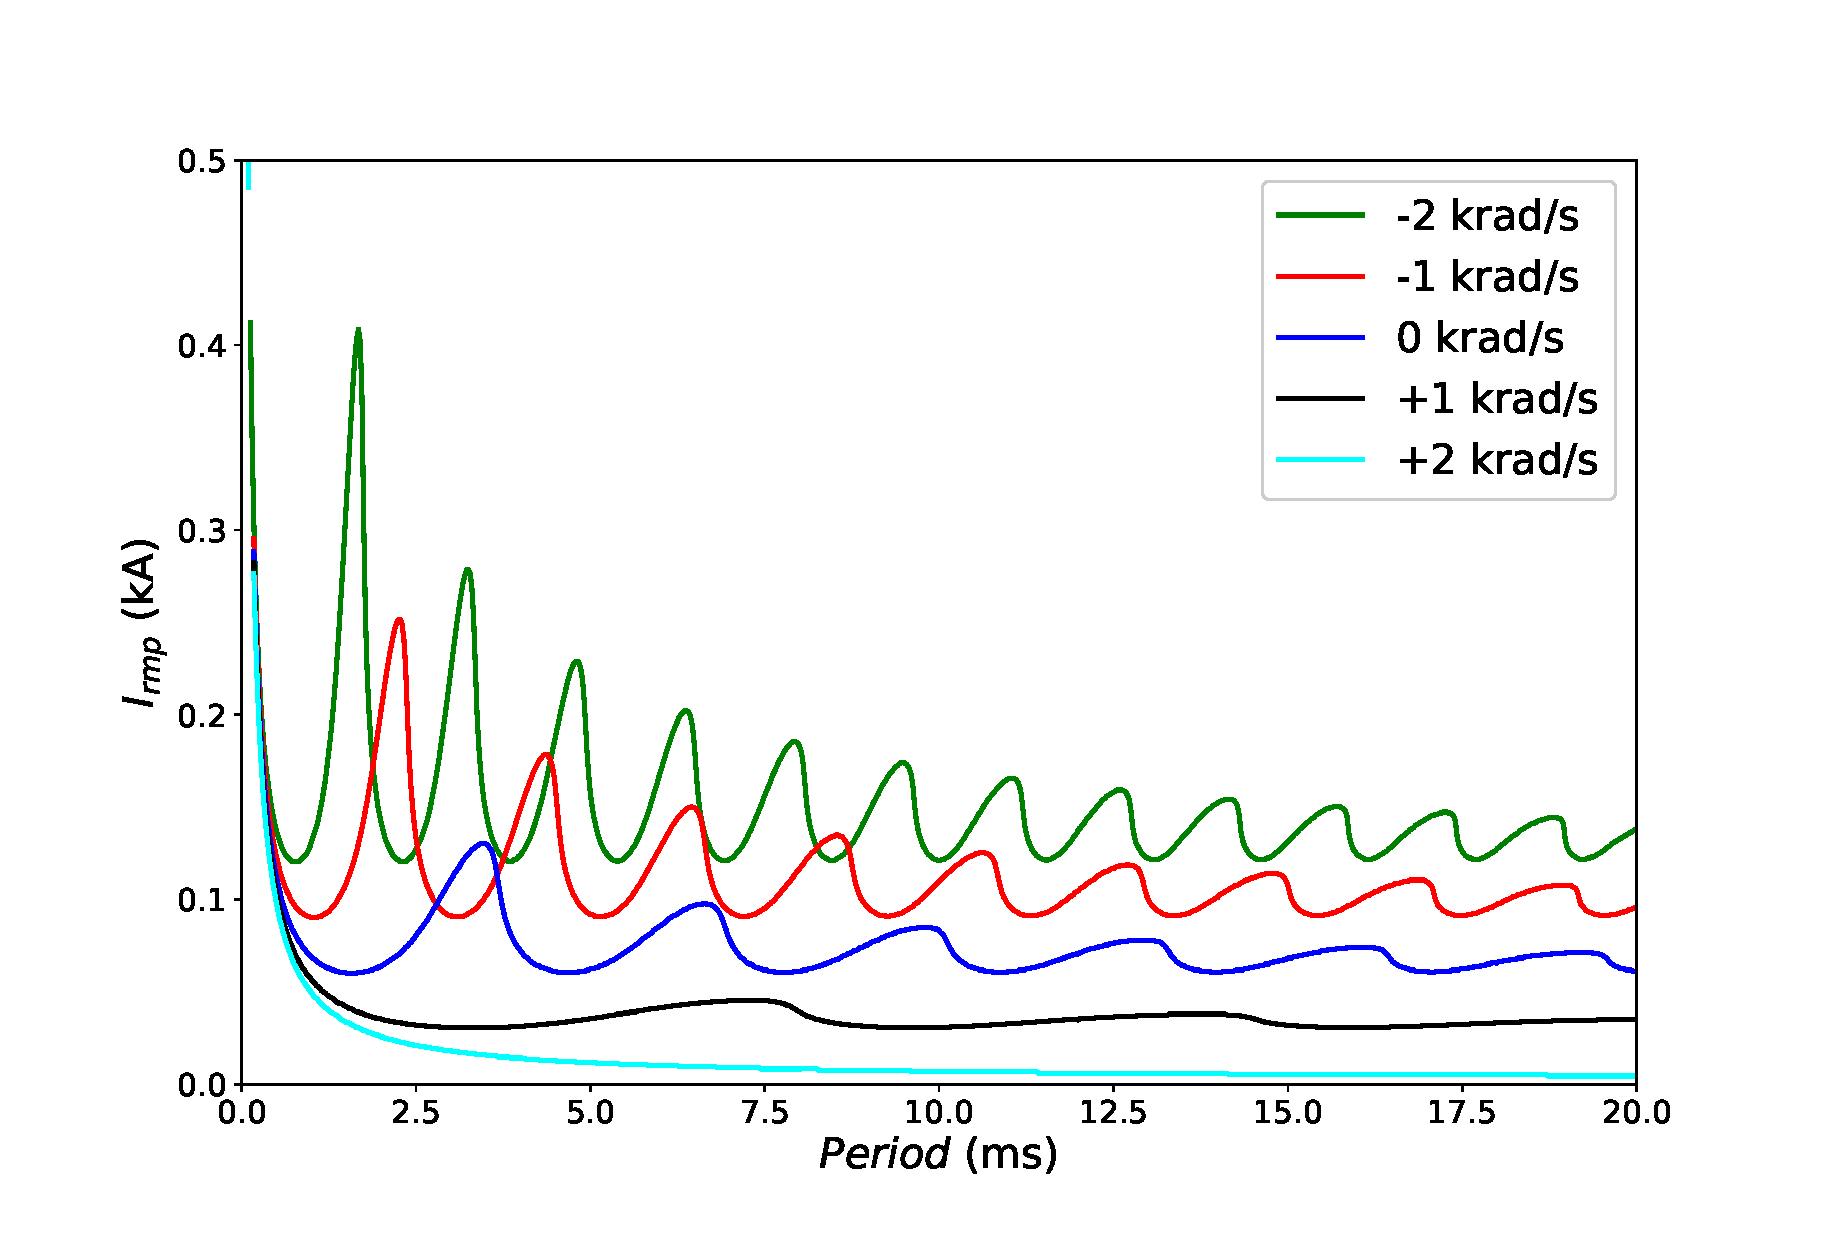
\includegraphics[width=\textwidth]{PeriodScan.eps}
\end{center}

\end{frame}

\begin{frame}
\frametitle{NSTX Shot 127317: Period/Frequency Scan}
\begin{itemize}
\item Clear from figure that as we move towards natural frequency (\blue{$2.1$ krad/s}), critical RMP current
is reduced, and oscillations become smaller in amplitude and longer in period.
\item Conversely, as we move away from  natural frequency, critical RMP current
increases, and oscillations become larger in amplitude and shorter in period.

\end{itemize}
\end{frame}

\begin{frame}
\frametitle{NSTX Shot 127317: Frequency Scan}

\begin{center}
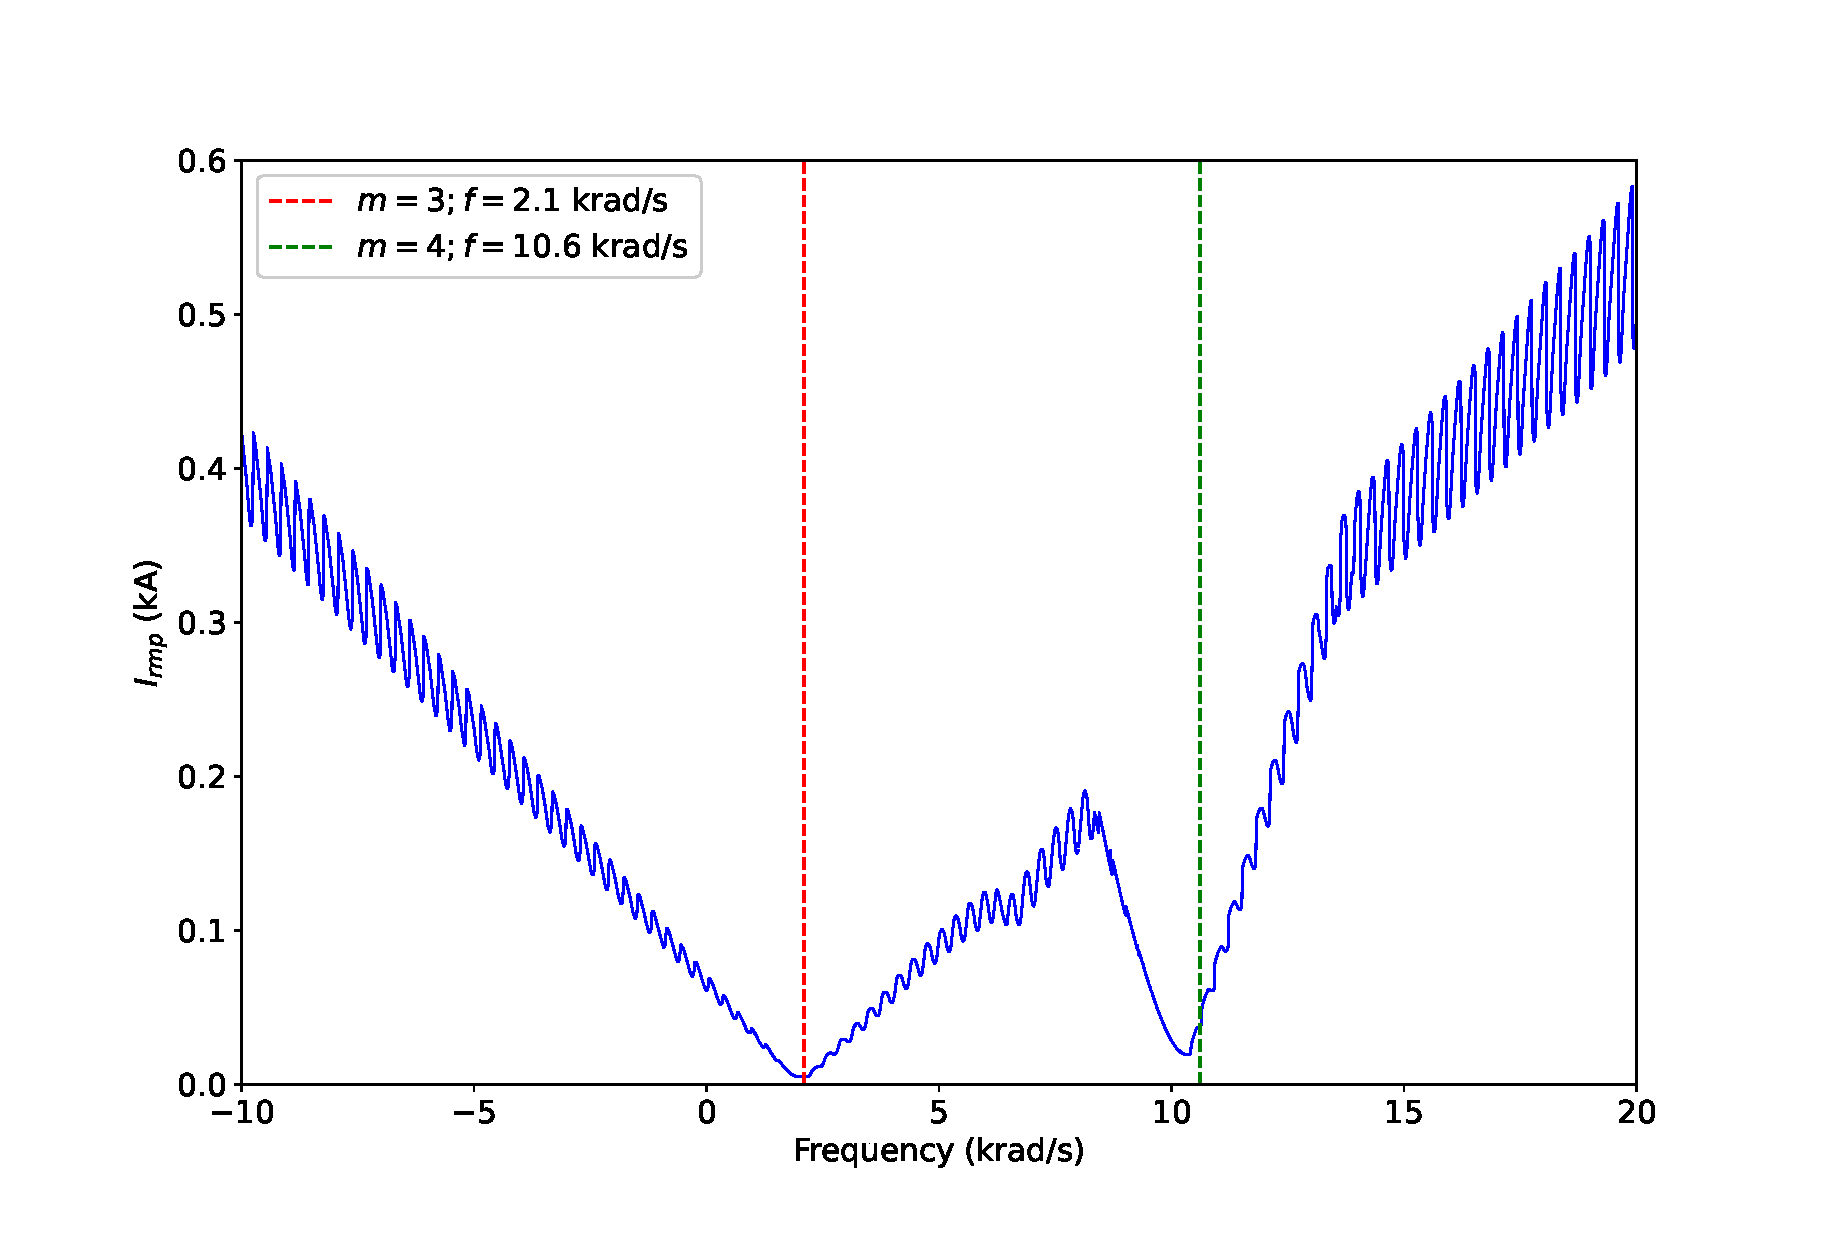
\includegraphics[width=\textwidth]{FrequencyScan.eps}
\end{center}

\end{frame}

\begin{frame}
\frametitle{NSTX Shot 127317: Frequency Scan}
\begin{itemize}
\item Figure shows critical RMP current required to trigger NTM, for pulse of period \blue{20 ms}, as
function of pulse frequency. 
\item Critical current minimized when pulse frequency matches natural frequency of either of potentially
unstable NTMs. 

\end{itemize}
\end{frame}

\begin{frame}
\frametitle{NSTX Shot 127317: Frequency Scan}

\begin{center}
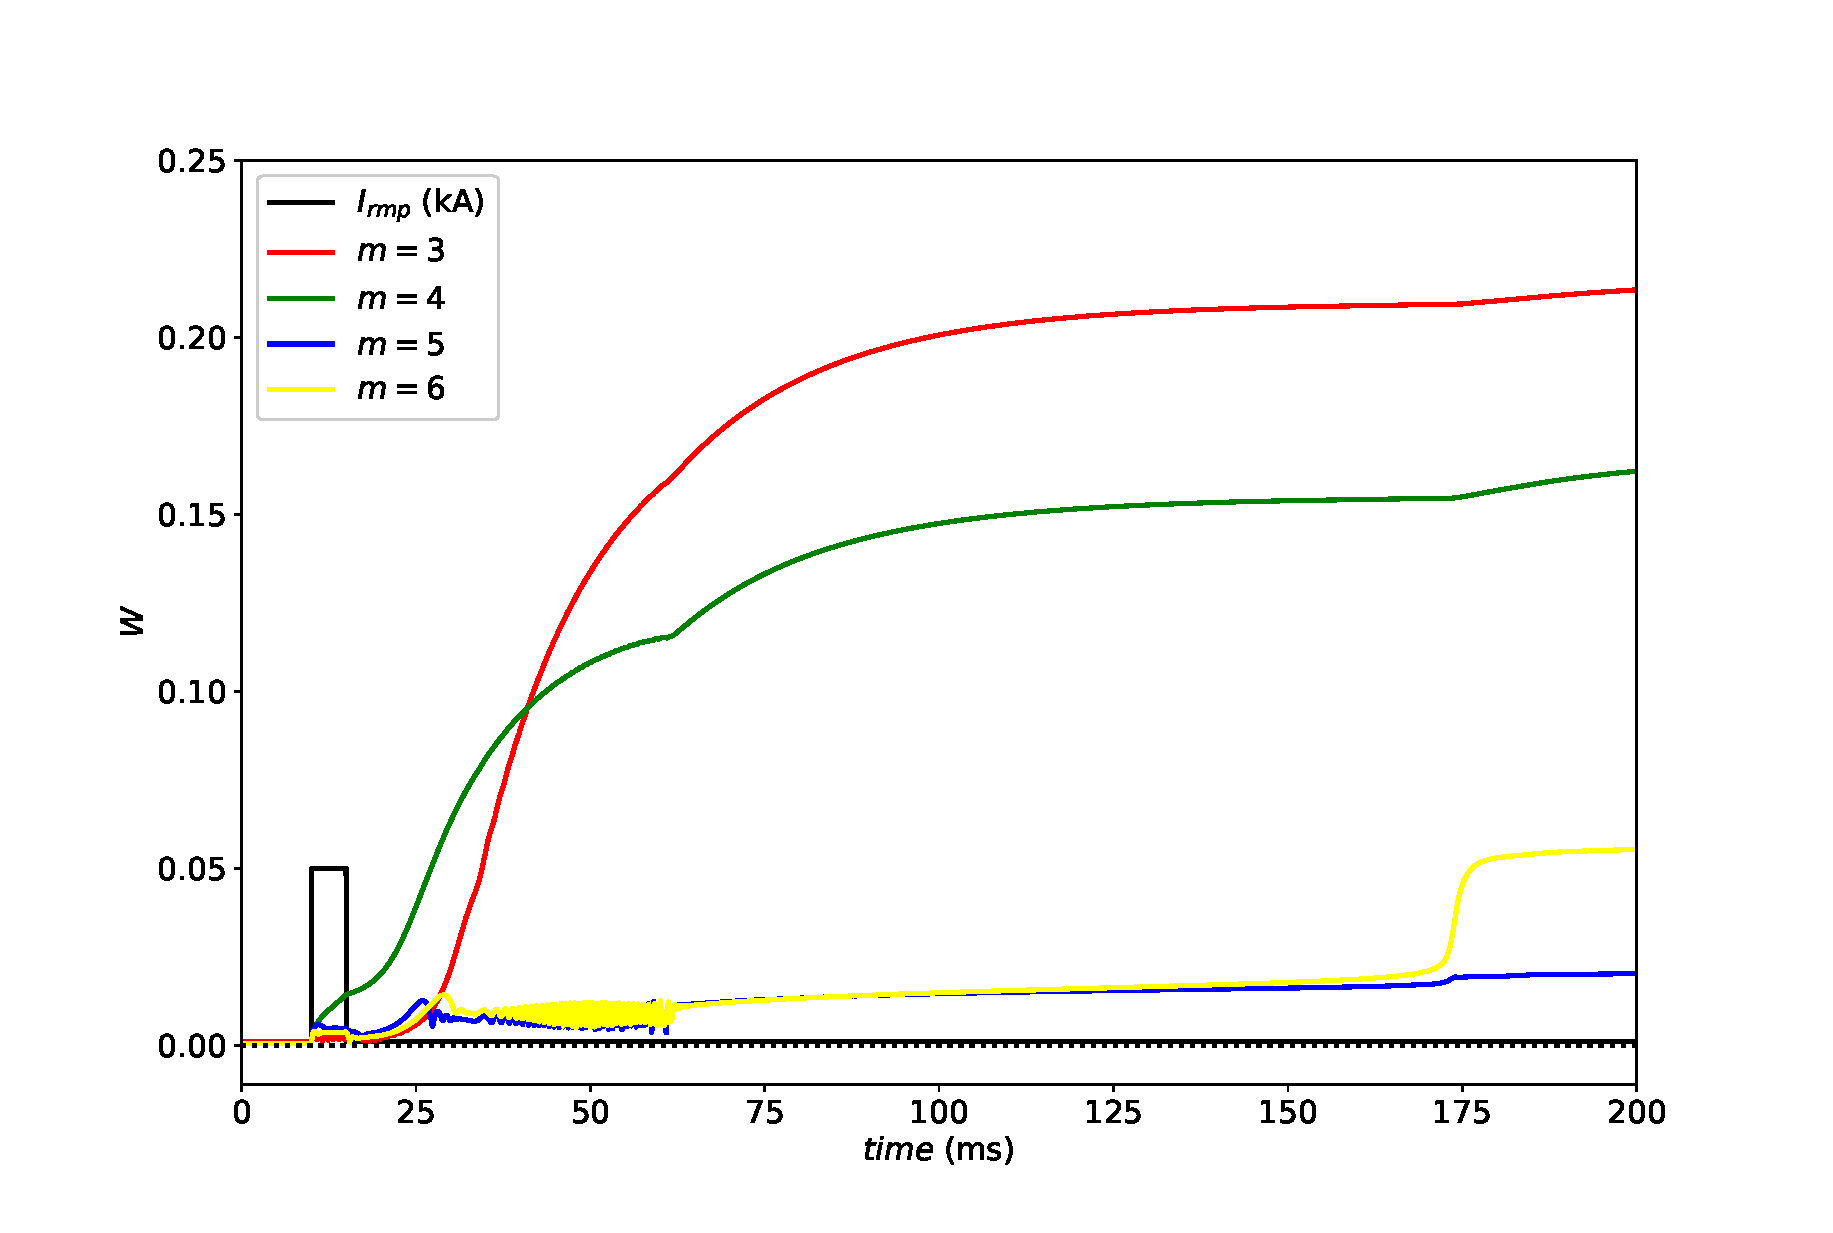
\includegraphics[width=\textwidth]{Waveform2.eps}
\end{center}

\end{frame}

\begin{frame}
\frametitle{NSTX Shot 127317: Frequency Scan}
\begin{itemize}
\item Figure shows effect of pulse whose frequency matches \blue{$m=4$} NTMs natural frequency.
\item Pulse triggers both \blue{$m=4$} and \blue{$m=3$} NTMs.
\item Two NTMs lock. Subsequently, other mode lock to NTMs. 
\item Note that pulse that triggers this catastrophic series of events would have triggered nothing
if its frequency were zero. 
\end{itemize}
\end{frame}

\begin{frame}
\frametitle{Conclusions}
\begin{itemize}
\item Have investigated what properties of multi-harmonic magnetic perturbation make it effective at
triggering NTMs.
\item Have found that by far the most important property of the perturbation is its \red{frequency}.
\item If frequency close to natural frequency of potentially unstable NTM then it is easy to trigger associated NTM.
\item If frequency is far from natural frequencies of potentially unstable NTMs then perturbation is ineffective at
triggering NTMs.
\end{itemize}
\end{frame}

\end{document}